The trigger system in the barrel region depends on RPC's that are arranged in three concentric cylindrical layers about the beam axis, and are referred to as the three trigger stations. The RPC's are a gaseous parallel electrode-plate detector with no wires, consisting of two resistive plates made up phenolic-melaminic plastic laminate separated from one another by 2 mm using insulating spacers. An electric field of approximately 4.9 kV/mm is applied between the plates causing ionized particles or free electrons to accelerate towards the anode. These particles gain energy, ionizing other particles creating a so-called avalanche effect. The resulting signal is readout via capacitive coupling to metallic strips mounted on the outer surface of the plates. At the nominal operating voltage of 9.8 kV, the typical signal width is about 5 ns. The full RPC system includes approximately 3,800 gas volumes and 385,000 readout channels. The gas mixture used in the RPC's consist of $C_2H_2F_4$ (94.7\%), Iso-$C_4H_{10}$ (5\%), and $SF_6$ (0.3\%) due to their low operating voltage, non-flammability and low costs, while maintaining a stable avalanche response. In the middle and outer layers of the barrel region, RPC's and positioned around the MDT's. The middle layer, RPC's are positioned both in front of, and behind the MDT's, while the outer layer they are positioned either in front (small chamber) or behind (large chamber). A diagram of this can be seen in Figure~\ref{fig:atlas_mdt_rpc_sandwich}.

\begin{figure}[htp]
    \centering
    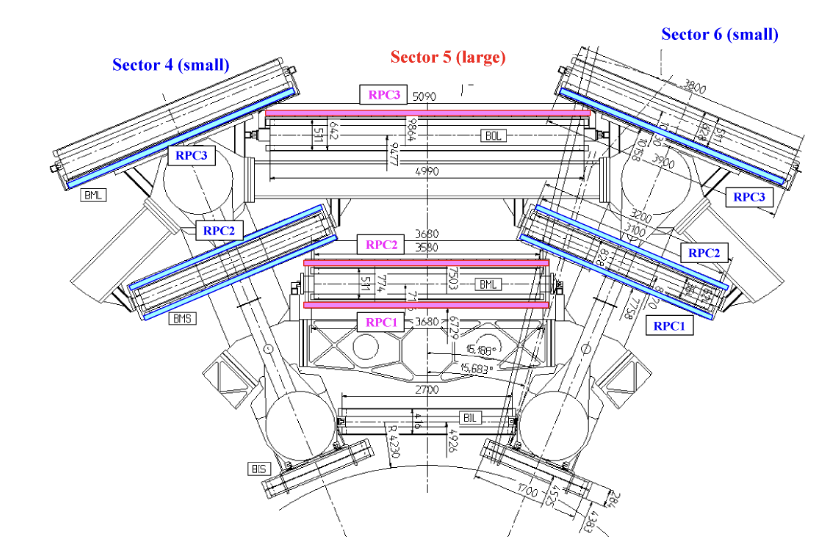
\includegraphics[width=0.8\textwidth]{figures/atlas/atlas_mdt_rpc_sandwich.png}
    \caption{Layout of the RPC and MDT system in the barrel region. The RPC's are placed in front of and behind the MDT's in the middle layer, and either in front of or behind the MDT's in the outer layer. Taken from~\cite{atlas_collaboration_paper}.}\label{fig:atlas_mdt_rpc_sandwich}
\end{figure}
